\documentclass[]{article}
\usepackage{lmodern}
\usepackage{amssymb,amsmath}
\usepackage{ifxetex,ifluatex}
\usepackage{fixltx2e} % provides \textsubscript
\ifnum 0\ifxetex 1\fi\ifluatex 1\fi=0 % if pdftex
  \usepackage[T1]{fontenc}
  \usepackage[utf8]{inputenc}
\else % if luatex or xelatex
  \ifxetex
    \usepackage{mathspec}
  \else
    \usepackage{fontspec}
  \fi
  \defaultfontfeatures{Ligatures=TeX,Scale=MatchLowercase}
\fi
% use upquote if available, for straight quotes in verbatim environments
\IfFileExists{upquote.sty}{\usepackage{upquote}}{}
% use microtype if available
\IfFileExists{microtype.sty}{%
\usepackage{microtype}
\UseMicrotypeSet[protrusion]{basicmath} % disable protrusion for tt fonts
}{}
\usepackage[margin=1in]{geometry}
\usepackage{hyperref}
\hypersetup{unicode=true,
            pdftitle={r\_49: Facebook Relationship Prediction},
            pdfauthor={JHU Team},
            pdfborder={0 0 0},
            breaklinks=true}
\urlstyle{same}  % don't use monospace font for urls
\usepackage{color}
\usepackage{fancyvrb}
\newcommand{\VerbBar}{|}
\newcommand{\VERB}{\Verb[commandchars=\\\{\}]}
\DefineVerbatimEnvironment{Highlighting}{Verbatim}{commandchars=\\\{\}}
% Add ',fontsize=\small' for more characters per line
\usepackage{framed}
\definecolor{shadecolor}{RGB}{248,248,248}
\newenvironment{Shaded}{\begin{snugshade}}{\end{snugshade}}
\newcommand{\KeywordTok}[1]{\textcolor[rgb]{0.13,0.29,0.53}{\textbf{#1}}}
\newcommand{\DataTypeTok}[1]{\textcolor[rgb]{0.13,0.29,0.53}{#1}}
\newcommand{\DecValTok}[1]{\textcolor[rgb]{0.00,0.00,0.81}{#1}}
\newcommand{\BaseNTok}[1]{\textcolor[rgb]{0.00,0.00,0.81}{#1}}
\newcommand{\FloatTok}[1]{\textcolor[rgb]{0.00,0.00,0.81}{#1}}
\newcommand{\ConstantTok}[1]{\textcolor[rgb]{0.00,0.00,0.00}{#1}}
\newcommand{\CharTok}[1]{\textcolor[rgb]{0.31,0.60,0.02}{#1}}
\newcommand{\SpecialCharTok}[1]{\textcolor[rgb]{0.00,0.00,0.00}{#1}}
\newcommand{\StringTok}[1]{\textcolor[rgb]{0.31,0.60,0.02}{#1}}
\newcommand{\VerbatimStringTok}[1]{\textcolor[rgb]{0.31,0.60,0.02}{#1}}
\newcommand{\SpecialStringTok}[1]{\textcolor[rgb]{0.31,0.60,0.02}{#1}}
\newcommand{\ImportTok}[1]{#1}
\newcommand{\CommentTok}[1]{\textcolor[rgb]{0.56,0.35,0.01}{\textit{#1}}}
\newcommand{\DocumentationTok}[1]{\textcolor[rgb]{0.56,0.35,0.01}{\textbf{\textit{#1}}}}
\newcommand{\AnnotationTok}[1]{\textcolor[rgb]{0.56,0.35,0.01}{\textbf{\textit{#1}}}}
\newcommand{\CommentVarTok}[1]{\textcolor[rgb]{0.56,0.35,0.01}{\textbf{\textit{#1}}}}
\newcommand{\OtherTok}[1]{\textcolor[rgb]{0.56,0.35,0.01}{#1}}
\newcommand{\FunctionTok}[1]{\textcolor[rgb]{0.00,0.00,0.00}{#1}}
\newcommand{\VariableTok}[1]{\textcolor[rgb]{0.00,0.00,0.00}{#1}}
\newcommand{\ControlFlowTok}[1]{\textcolor[rgb]{0.13,0.29,0.53}{\textbf{#1}}}
\newcommand{\OperatorTok}[1]{\textcolor[rgb]{0.81,0.36,0.00}{\textbf{#1}}}
\newcommand{\BuiltInTok}[1]{#1}
\newcommand{\ExtensionTok}[1]{#1}
\newcommand{\PreprocessorTok}[1]{\textcolor[rgb]{0.56,0.35,0.01}{\textit{#1}}}
\newcommand{\AttributeTok}[1]{\textcolor[rgb]{0.77,0.63,0.00}{#1}}
\newcommand{\RegionMarkerTok}[1]{#1}
\newcommand{\InformationTok}[1]{\textcolor[rgb]{0.56,0.35,0.01}{\textbf{\textit{#1}}}}
\newcommand{\WarningTok}[1]{\textcolor[rgb]{0.56,0.35,0.01}{\textbf{\textit{#1}}}}
\newcommand{\AlertTok}[1]{\textcolor[rgb]{0.94,0.16,0.16}{#1}}
\newcommand{\ErrorTok}[1]{\textcolor[rgb]{0.64,0.00,0.00}{\textbf{#1}}}
\newcommand{\NormalTok}[1]{#1}
\usepackage{graphicx,grffile}
\makeatletter
\def\maxwidth{\ifdim\Gin@nat@width>\linewidth\linewidth\else\Gin@nat@width\fi}
\def\maxheight{\ifdim\Gin@nat@height>\textheight\textheight\else\Gin@nat@height\fi}
\makeatother
% Scale images if necessary, so that they will not overflow the page
% margins by default, and it is still possible to overwrite the defaults
% using explicit options in \includegraphics[width, height, ...]{}
\setkeys{Gin}{width=\maxwidth,height=\maxheight,keepaspectratio}
\usepackage[normalem]{ulem}
% avoid problems with \sout in headers with hyperref:
\pdfstringdefDisableCommands{\renewcommand{\sout}{}}
\IfFileExists{parskip.sty}{%
\usepackage{parskip}
}{% else
\setlength{\parindent}{0pt}
\setlength{\parskip}{6pt plus 2pt minus 1pt}
}
\setlength{\emergencystretch}{3em}  % prevent overfull lines
\providecommand{\tightlist}{%
  \setlength{\itemsep}{0pt}\setlength{\parskip}{0pt}}
\setcounter{secnumdepth}{5}
% Redefines (sub)paragraphs to behave more like sections
\ifx\paragraph\undefined\else
\let\oldparagraph\paragraph
\renewcommand{\paragraph}[1]{\oldparagraph{#1}\mbox{}}
\fi
\ifx\subparagraph\undefined\else
\let\oldsubparagraph\subparagraph
\renewcommand{\subparagraph}[1]{\oldsubparagraph{#1}\mbox{}}
\fi

%%% Use protect on footnotes to avoid problems with footnotes in titles
\let\rmarkdownfootnote\footnote%
\def\footnote{\protect\rmarkdownfootnote}

%%% Change title format to be more compact
\usepackage{titling}

% Create subtitle command for use in maketitle
\newcommand{\subtitle}[1]{
  \posttitle{
    \begin{center}\large#1\end{center}
    }
}

\setlength{\droptitle}{-2em}
  \title{\texttt{r\_49}: Facebook Relationship Prediction}
  \pretitle{\vspace{\droptitle}\centering\huge}
  \posttitle{\par}
  \author{JHU Team}
  \preauthor{\centering\large\emph}
  \postauthor{\par}
  \predate{\centering\large\emph}
  \postdate{\par}
  \date{2017-09-17}


\begin{document}
\maketitle

{
\setcounter{tocdepth}{2}
\tableofcontents
}
\section{Problem}\label{problem}

GM250\_seed is an instance of the Graph Matching problem.\\
In this problem two graphs are given. \texttt{G1} and \texttt{G2}.\\
A partial map between nodes of \texttt{G1} and \texttt{G2} are provided
in the train data.\\
The task is to predict the mapping between the unmapped nodes in the
test data.

\section{Data}\label{data}

Data for GM250\_seed consists of two graphs in raw\_data dir:

\begin{itemize}
\tightlist
\item
  \texttt{G1.gml}: attributed undirected graph; \sout{250} 755 nodes;
  5138 edges; \sout{12} 4 features for each node
\item
  \texttt{G2.gml}: attributed undirected graph; \sout{124} 755 nodes;
  \sout{324} 5138 edges; \sout{12} 4 features for each node
\item
  \texttt{trainData.csv} contains \texttt{G1} nodes and
  \texttt{trainTargets.csv} contains \texttt{G2} nodes. Together, they
  constitute 151 known mappings.
\item
  \sout{\texttt{testData.csv} contains \texttt{G2} nodes, for which the
  mappings have to be predicted in \texttt{testTargets.csv}}
\end{itemize}

\begin{Shaded}
\begin{Highlighting}[]
\KeywordTok{suppressMessages}\NormalTok{(}\KeywordTok{library}\NormalTok{(tidyverse))}
\KeywordTok{suppressMessages}\NormalTok{(}\KeywordTok{library}\NormalTok{(igraph))}
\KeywordTok{suppressMessages}\NormalTok{(}\KeywordTok{library}\NormalTok{(Matrix))}
\KeywordTok{suppressMessages}\NormalTok{(}\KeywordTok{library}\NormalTok{(VN))}

\NormalTok{g1file <-}\StringTok{ "http://www.cis.jhu.edu/~parky/D3M/r49/data/raw_data/G1.gml"}
\NormalTok{g2file <-}\StringTok{ "http://www.cis.jhu.edu/~parky/D3M/r49/data/raw_data/G2.gml"}

\NormalTok{g1 <-}\StringTok{ }\KeywordTok{read_graph}\NormalTok{(g1file,}\DataTypeTok{format =} \StringTok{"gml"}\NormalTok{); }\KeywordTok{summary}\NormalTok{(g1); }\KeywordTok{is.connected}\NormalTok{(g1)}
\end{Highlighting}
\end{Shaded}

\begin{verbatim}
# IGRAPH 3a1d7fc U--- 1000 5521 -- 
# + attr: id (v/n), label (v/n), nodeID (v/n), f0 (v/n), f1 (v/n),
# | f2 (v/n), f3 (v/n), f4 (v/n), class (v/n)
\end{verbatim}

\begin{verbatim}
# [1] FALSE
\end{verbatim}

\begin{Shaded}
\begin{Highlighting}[]
\NormalTok{g2 <-}\StringTok{ }\KeywordTok{read_graph}\NormalTok{(g2file,}\DataTypeTok{format =} \StringTok{"gml"}\NormalTok{); }\KeywordTok{summary}\NormalTok{(g2); }\KeywordTok{is.connected}\NormalTok{(g2)}
\end{Highlighting}
\end{Shaded}

\begin{verbatim}
# IGRAPH 1e2817c U--- 755 5138 -- 
# + attr: id (v/n), label (v/n), f0 (v/n), f1 (v/n), f2 (v/n), f3
# | (v/n), f4 (v/n), class (v/n), nodeID (v/n)
\end{verbatim}

\begin{verbatim}
# [1] TRUE
\end{verbatim}

\begin{Shaded}
\begin{Highlighting}[]
\CommentTok{# find lcc of g1}
\NormalTok{cl <-}\StringTok{ }\NormalTok{igraph}\OperatorTok{::}\KeywordTok{clusters}\NormalTok{(g1)}
\NormalTok{g1 <-}\StringTok{ }\KeywordTok{induced.subgraph}\NormalTok{(g1, }\KeywordTok{which}\NormalTok{(cl}\OperatorTok{$}\NormalTok{membership }\OperatorTok{==}\StringTok{ }\KeywordTok{which.max}\NormalTok{(cl}\OperatorTok{$}\NormalTok{csize)))}
\KeywordTok{summary}\NormalTok{(g1)}
\end{Highlighting}
\end{Shaded}

\begin{verbatim}
# IGRAPH 7e0198c U--- 755 5138 -- 
# + attr: id (v/n), label (v/n), nodeID (v/n), f0 (v/n), f1 (v/n),
# | f2 (v/n), f3 (v/n), f4 (v/n), class (v/n)
\end{verbatim}

\begin{Shaded}
\begin{Highlighting}[]
\KeywordTok{isomorphic}\NormalTok{(g1, g2)}
\end{Highlighting}
\end{Shaded}

\begin{verbatim}
# [1] TRUE
\end{verbatim}

\begin{Shaded}
\begin{Highlighting}[]
\CommentTok{# id == nodeID}
\CommentTok{# revise node ids}
\KeywordTok{V}\NormalTok{(g1)}\OperatorTok{$}\NormalTok{id <-}\StringTok{ }\DecValTok{1}\OperatorTok{:}\KeywordTok{vcount}\NormalTok{(g1)}
\KeywordTok{V}\NormalTok{(g2)}\OperatorTok{$}\NormalTok{id <-}\StringTok{ }\DecValTok{1}\OperatorTok{:}\KeywordTok{vcount}\NormalTok{(g2)}
\end{Highlighting}
\end{Shaded}

\begin{Shaded}
\begin{Highlighting}[]
\NormalTok{train1 <-}\StringTok{ }\KeywordTok{read_csv}\NormalTok{(}\StringTok{"http://www.cis.jhu.edu/~parky/D3M/r49/data/trainData.csv"}\NormalTok{)}
\NormalTok{train2 <-}\StringTok{ }\KeywordTok{read_csv}\NormalTok{(}\StringTok{"http://www.cis.jhu.edu/~parky/D3M/r49/data/trainTargets.csv"}\NormalTok{)}
\CommentTok{#test <- read_csv("~/Dropbox/D3M/D3M/r49/solution/baseline/testTargets.csv")}
\NormalTok{train <-}\StringTok{ }\KeywordTok{left_join}\NormalTok{(train1,train2, }\DataTypeTok{by=}\StringTok{"d3mIndex"}\NormalTok{); train}
\end{Highlighting}
\end{Shaded}

\begin{verbatim}
# # A tibble: 151 x 5
#    d3mIndex graph.x G1.nodeID graph.y G2.nodeID
#       <int>   <chr>     <int>   <chr>     <int>
#  1        0  G1.gml         7  G2.gml        32
#  2        1  G1.gml       152  G2.gml       433
#  3        2  G1.gml       742  G2.gml       831
#  4        3  G1.gml        12  G2.gml       616
#  5        4  G1.gml       277  G2.gml       515
#  6        5  G1.gml       279  G2.gml       796
#  7        6  G1.gml       430  G2.gml       457
#  8        7  G1.gml        15  G2.gml       680
#  9        8  G1.gml       117  G2.gml       401
# 10        9  G1.gml       389  G2.gml       737
# # ... with 141 more rows
\end{verbatim}

\begin{Shaded}
\begin{Highlighting}[]
\CommentTok{# rearrange the graphs so that seeds are the first m vertices}
\NormalTok{matched.id1 <-}\StringTok{ }\KeywordTok{match}\NormalTok{(train}\OperatorTok{$}\NormalTok{G1.nodeID, }\KeywordTok{V}\NormalTok{(g1)}\OperatorTok{$}\NormalTok{nodeID) }\CommentTok{# 151}
\NormalTok{perm.g1 <-}\StringTok{ }\KeywordTok{invPerm}\NormalTok{(}\KeywordTok{c}\NormalTok{(matched.id1, (}\DecValTok{1}\OperatorTok{:}\KeywordTok{vcount}\NormalTok{(g1))[}\OperatorTok{-}\NormalTok{matched.id1]))}
\NormalTok{matched.id2 <-}\StringTok{ }\KeywordTok{unique}\NormalTok{(}\KeywordTok{match}\NormalTok{(train}\OperatorTok{$}\NormalTok{G2.nodeID, }\KeywordTok{V}\NormalTok{(g2)}\OperatorTok{$}\NormalTok{nodeID)) }\CommentTok{# 145}
\NormalTok{perm.g2 <-}\StringTok{ }\KeywordTok{invPerm}\NormalTok{(}\KeywordTok{c}\NormalTok{(matched.id2, (}\DecValTok{1}\OperatorTok{:}\KeywordTok{vcount}\NormalTok{(g2))[}\OperatorTok{-}\NormalTok{matched.id2]))}
\NormalTok{g1.new <-}\StringTok{ }\KeywordTok{permute.vertices}\NormalTok{(g1, perm.g1); }\KeywordTok{head}\NormalTok{(}\KeywordTok{V}\NormalTok{(g1.new)}\OperatorTok{$}\NormalTok{nodeID, }\DecValTok{10}\NormalTok{)}
\end{Highlighting}
\end{Shaded}

\begin{verbatim}
#  [1]   7 152 742  12 277 279 430  15 117 389
\end{verbatim}

\begin{Shaded}
\begin{Highlighting}[]
\NormalTok{g2.new <-}\StringTok{ }\KeywordTok{permute.vertices}\NormalTok{(g2, perm.g2); }\KeywordTok{head}\NormalTok{(}\KeywordTok{V}\NormalTok{(g2.new)}\OperatorTok{$}\NormalTok{nodeID, }\DecValTok{10}\NormalTok{)}
\end{Highlighting}
\end{Shaded}

\begin{verbatim}
#  [1]  32 433 831 616 515 796 457 680 401 737
\end{verbatim}

\begin{Shaded}
\begin{Highlighting}[]
\NormalTok{g2.sub <-}\StringTok{ }\KeywordTok{induced.subgraph}\NormalTok{(g2.new, }\DecValTok{1}\OperatorTok{:}\KeywordTok{nrow}\NormalTok{(train)); }\KeywordTok{summary}\NormalTok{(g2.sub)}
\end{Highlighting}
\end{Shaded}

\begin{verbatim}
# IGRAPH 39b70ab U--- 151 215 -- 
# + attr: id (v/n), label (v/n), f0 (v/n), f1 (v/n), f2 (v/n), f3
# | (v/n), f4 (v/n), class (v/n), nodeID (v/n)
\end{verbatim}

\section{Seeded Graph Matching}\label{seeded-graph-matching}

So, \texttt{m} = 151 correspondence are given.\\
We will use the first \(s = \{0,30,60,90,120, 150\}\) vertices as seeds
and repeat the process 100 times to see the matching performance.

\begin{quote}
On Sep 9, 2017, at 12:18 PM, Vince Lyzinski
\href{mailto:vincelyzinski@gmail.com}{\nolinkurl{vincelyzinski@gmail.com}}
wrote:

hard seeding enforces the seeds throughout the problem (they can't
change), while soft seeding just initializes at the seeds, but allows
them to change in the course of the optimization
\end{quote}

\begin{Shaded}
\begin{Highlighting}[]
\KeywordTok{set.seed}\NormalTok{(}\DecValTok{12345}\NormalTok{)}

\NormalTok{A1 <-}\StringTok{ }\KeywordTok{as.matrix}\NormalTok{(g1.new[])}
\NormalTok{A2 <-}\StringTok{ }\KeywordTok{as.matrix}\NormalTok{(g2.new[])}
\NormalTok{n <-}\StringTok{ }\KeywordTok{nrow}\NormalTok{(A1)}
\NormalTok{m <-}\StringTok{ }\KeywordTok{nrow}\NormalTok{(train)}
\NormalTok{gamma <-}\StringTok{ }\DecValTok{1}

\NormalTok{nmc <-}\StringTok{ }\DecValTok{100}
\NormalTok{niter <-}\StringTok{ }\DecValTok{100}
\NormalTok{svec <-}\StringTok{ }\KeywordTok{seq}\NormalTok{(}\DecValTok{0}\NormalTok{, }\DecValTok{150}\NormalTok{, }\DataTypeTok{by=}\DecValTok{30}\NormalTok{)}
\end{Highlighting}
\end{Shaded}

\begin{Shaded}
\begin{Highlighting}[]
\NormalTok{method <-}\StringTok{ "soft"}
\NormalTok{nmc <-}\StringTok{ }\KeywordTok{ifelse}\NormalTok{(method}\OperatorTok{==}\StringTok{"soft"}\NormalTok{, }\DecValTok{100}\NormalTok{, }\DecValTok{1}\NormalTok{)}
\NormalTok{niter <-}\StringTok{ }\KeywordTok{ifelse}\NormalTok{(method}\OperatorTok{==}\StringTok{"soft"}\NormalTok{, }\DecValTok{100}\NormalTok{, }\DecValTok{30}\NormalTok{)}

\ControlFlowTok{for}\NormalTok{ (s }\ControlFlowTok{in}\NormalTok{ svec) \{}
    \KeywordTok{cat}\NormalTok{(}\StringTok{"Working on s = "}\NormalTok{, s, }\StringTok{"}\CharTok{\textbackslash{}n}\StringTok{"}\NormalTok{)}
\NormalTok{    mc <-}\StringTok{ }\KeywordTok{foreach}\NormalTok{ (}\DataTypeTok{i=}\DecValTok{1}\OperatorTok{:}\NormalTok{nmc) }\OperatorTok\StringTok{ }\NormalTok{\{}
\NormalTok{        ## S is a starting point for softseeding}
        \ControlFlowTok{if}\NormalTok{ (method}\OperatorTok{==}\StringTok{"soft"}\NormalTok{) \{}
\NormalTok{            M <-}\StringTok{ }\KeywordTok{rsp}\NormalTok{(n}\OperatorTok{-}\NormalTok{s,gamma)}
\NormalTok{            S <-}\StringTok{ }\KeywordTok{diag}\NormalTok{(n);}
\NormalTok{            S[(s}\OperatorTok{+}\DecValTok{1}\NormalTok{)}\OperatorTok{:}\NormalTok{n,(s}\OperatorTok{+}\DecValTok{1}\NormalTok{)}\OperatorTok{:}\NormalTok{n] <-}\StringTok{ }\NormalTok{M}
\NormalTok{            out <-}\StringTok{ }\KeywordTok{sgm}\NormalTok{(A2,A1,}\DecValTok{0}\NormalTok{,}\DataTypeTok{start=}\NormalTok{S,}\DataTypeTok{pad=}\DecValTok{0}\NormalTok{,}\DataTypeTok{iteration=}\NormalTok{niter)}
\NormalTok{        \} }\ControlFlowTok{else}\NormalTok{ \{ }\CommentTok{# "hard"}
\NormalTok{            S <-}\KeywordTok{matrix}\NormalTok{(}\DecValTok{1}\OperatorTok{/}\NormalTok{(n}\OperatorTok{-}\NormalTok{s), n}\OperatorTok{-}\NormalTok{s, n}\OperatorTok{-}\NormalTok{s) }
\NormalTok{            out <-}\StringTok{ }\KeywordTok{sgm}\NormalTok{(A2,A1,s,}\DataTypeTok{start=}\NormalTok{S,}\DataTypeTok{pad=}\DecValTok{0}\NormalTok{,}\DataTypeTok{iteration=}\NormalTok{niter)}
            \ControlFlowTok{if}\NormalTok{ (s }\OperatorTok{>}\StringTok{ }\DecValTok{0}\NormalTok{) \{}
\NormalTok{                out}\OperatorTok{$}\NormalTok{corr <-}\StringTok{ }\KeywordTok{c}\NormalTok{(}\DecValTok{1}\OperatorTok{:}\NormalTok{s,out}\OperatorTok{$}\NormalTok{corr)  }
\NormalTok{            \}}
\NormalTok{        \}}
        
\NormalTok{        newA2 <-}\StringTok{ }\NormalTok{out}\OperatorTok{$}\NormalTok{P }\OperatorTok\StringTok{ }\NormalTok{A1 }\OperatorTok\StringTok{ }\KeywordTok{t}\NormalTok{(out}\OperatorTok{$}\NormalTok{P)}
\NormalTok{        f <-}\StringTok{ }\KeywordTok{norm}\NormalTok{(A2[}\DecValTok{1}\OperatorTok{:}\NormalTok{m,}\DecValTok{1}\OperatorTok{:}\NormalTok{m]}\OperatorTok{-}\NormalTok{newA2[}\DecValTok{1}\OperatorTok{:}\NormalTok{m,}\DecValTok{1}\OperatorTok{:}\NormalTok{m], }\StringTok{"F"}\NormalTok{)}
\NormalTok{        matchV <-}\StringTok{ }\KeywordTok{sum}\NormalTok{(out}\OperatorTok{$}\NormalTok{corr[}\DecValTok{1}\OperatorTok{:}\NormalTok{m] }\OperatorTok{==}\StringTok{ }\DecValTok{1}\OperatorTok{:}\NormalTok{m)}
\NormalTok{        matchE <-}\StringTok{ }\KeywordTok{sum}\NormalTok{((A2[}\DecValTok{1}\OperatorTok{:}\NormalTok{m,}\DecValTok{1}\OperatorTok{:}\NormalTok{m]}\OperatorTok{+}\NormalTok{newA2[}\DecValTok{1}\OperatorTok{:}\NormalTok{m,}\DecValTok{1}\OperatorTok{:}\NormalTok{m])}\OperatorTok{>=}\DecValTok{2}\NormalTok{) }\OperatorTok{/}\StringTok{ }\DecValTok{2}
        \KeywordTok{c}\NormalTok{(matchV, matchE, f)}
\NormalTok{    \}}
    \KeywordTok{save}\NormalTok{(mc,n,m,nmc,s,gamma,}\DataTypeTok{file=}\KeywordTok{paste0}\NormalTok{(}\StringTok{"mc-r49-s"}\NormalTok{,s,}\StringTok{"-nmc"}\NormalTok{,nmc,}\StringTok{"-niter"}\NormalTok{,niter,}\StringTok{"-"}\NormalTok{,method,}\StringTok{".Rbin"}\NormalTok{))}
\NormalTok{\}}
\end{Highlighting}
\end{Shaded}

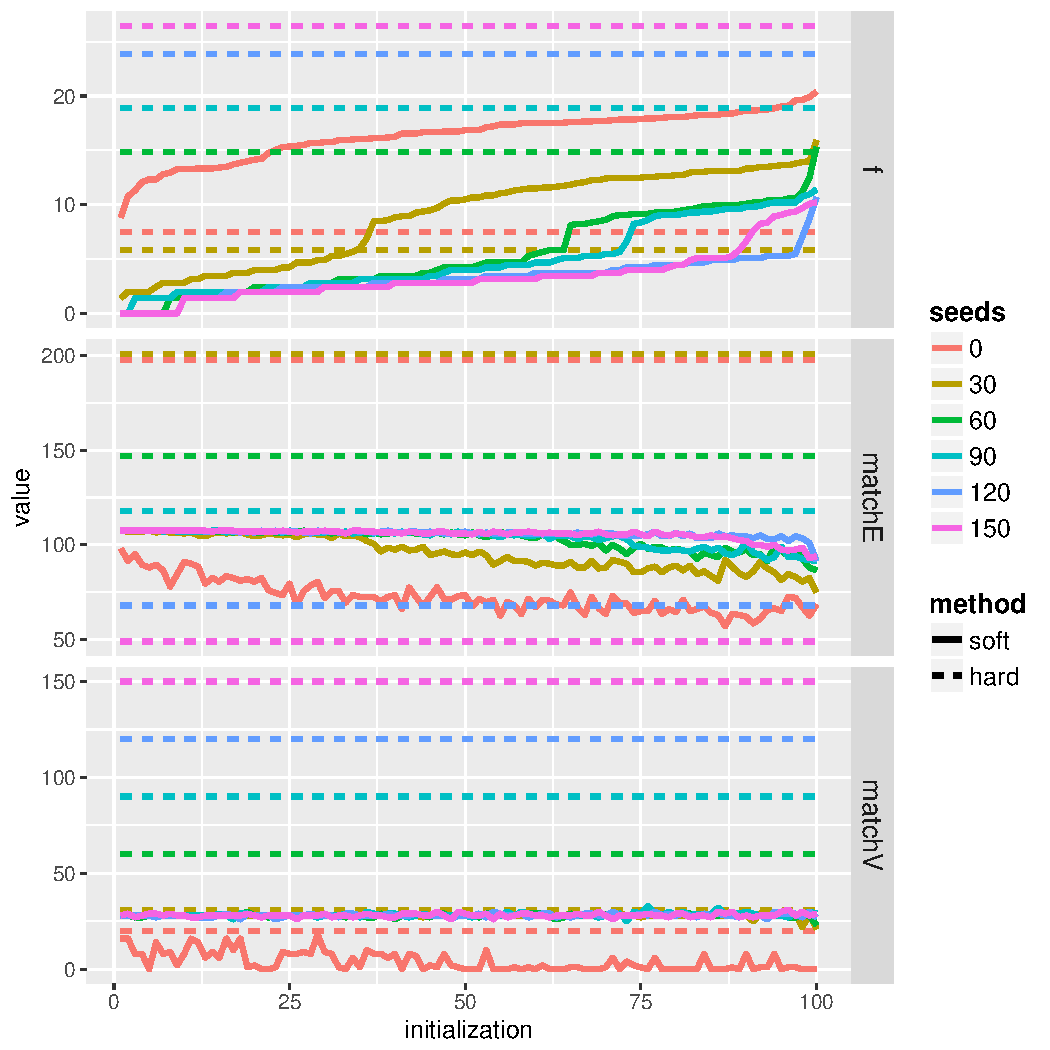
\includegraphics{r49_files/figure-latex/acollect21-1.pdf}


\end{document}
